% \chapter{Entorno de trabajo y experimentación}
%     \section{Elección del modelo de LLM e hiperparámetros óptimos}
%         \subsection{Modelo de LLM}
%             Elección de GPT-4.
%         \subsection{Hiperparámetros}
%             Temperatura, top\_p, ventana de contexto, número de \textit{tokens}, etc.
%     \section{Entorno de trabajo}
%         Distinguir entre el entorno de pruebas en chatGPT y el entorno delimitado de la API de OpenAI.
%         \subsection{Entorno de pruebas con chatbot}
%             Útil para experimentación libre. Pero no hay control de los hiperparámetros, las especificaciones pueden cambiar, lo que compromete la repibilidad de los resultados. No permite prompts en 2-steps.
%         \subsection{Entorno de trabajo con la API en Playground y en Python}
%             Hablar de LangChain y de la API de OpenAI.

% \chapter{Estrategias de \textit{prompting} para el diseño sonoro}
%     \section{\textit{Chain of Thoughts} y \textit{Structured Chain of Thoughts}}
%     \section{\textit{1-step} o \textit{2-step}}
%     \section{Uso de \textit{Self-debugging} y \textit{Chain of Verification}}

% \chapter{\textit{System Prompts} y \textit{User Prompts} diseñados para esta investigación}
%     \section{Diseños de \textit{System Prompts}}
%         Han de ser Pocos. Quizás entre 3 y 5. Describir los que se han elegido y lo que se espera de ellos.
%     \section{Diseños de \textit{User Prompts}}
%         Los prompts de usuario escogidos para solicitar al modelo la generación de sonidos y texturas sonoras. Los prompts no deben ser muchos, para poder llevar a cabo la investigación en un tiempo razonable. Deben abarcar diveras técnicas de síntesis, la creación de diversas texturas descritas en lenguaje natural, y la aplicación de teoremas matemáticos, principios físicos, o inspiracion en otras artes, como la pintura o la literatura para la generación sonora.



\chapter{Elección de lenguajes de programación musical para este trabajo}

% \defaultFontEpigraph{Transcription Is All You Need\dots}{\cite{hungTranscriptionAllYou2020}}
\defaultFontEpigraph{Transcription Is All You Need\dots}{Hung, Wichern, y Roux (2020)}

Existen en la actualidad numerosos lenguajes de programación musicales, cada uno con sus propias características y orientados a diferentes propósitos. En este capítulo se describen los lenguajes de programación musicales más relevantes, comparando sus características, para finalmente elegir los lenguajes que se utilizarán en esta investigación.

Los lenguajes de programación musicales abarcan tanto la generación sonora por medio de todo tipo de síntesis, como la manipulación de archivos de audio, la composición musical, la creación de interfaces de usuario, la creación de instalaciones sonoras, la notación musical, etc. No se pretende en este capítulo hacer una descripción exhaustiva de todos los lenguajes de programación musicales existentes, sino más bien una descripción de los lenguajes más relevantes, y que han sido tenidos en cuenta de algún modo en este trabajo. 

\section{Música en código de programación}

Una característica común a los lenguajes de programación musicales es el hecho de que su representación simbólica se realiza por medio de código de programación, en texto plano, y por tanto, son lenguajes formales, con una sintaxis y una semántica definidas. Esto significa que son lenguajes que pueden ser generados por un modelo de lenguaje natural, como los LLM, incluso si no han sido entrenados específicamente en estos lenguajes. Esto es importante, ya que permite que los LLM puedan generar código de estos lenguajes, y por tanto, que puedan generar sonidos y música de un modo indirecto. Los LLM, en su prentrenamiento, han sido entrenados con todo tipo de código, incluyendo lenguajes con propósitos musicales o sonoros. Aunque no podemos esperar que los LLM tengan tanta destreza en Csound como en Python, sí podemos esperar que sean capaces de generar código de Csound, y que este código sea correcto, y que por tanto, pueda ser ejecutado para generar sonidos. Otra cosa es que el código generado sea interesante, o que el sonido generado sea interesante, ni siquiera que el código generado tenga sentido musical. No obstante, explorar esta capacidad de creación musical por medio de la generación de código es uno de los objetivos de esta investigación. La figura \ref{fig:hola_mundo} muestra un \textit{¡Hola, mundo!}\footnote{Un \textit{¡Hola, mundo!}, o, más conocido como \textit{Hello, World!}, es un programa informático mínimo de un lenguaje de programación, el cual lo único que hace es imprimir en pantalla el texto <<¡Hola, Mundo!>>, con una finalidad pedagógica. Por extensión, un \textit{¡Hola, Mundo!} de un lenguaje musical sería aquel que produce un sonido simple, como una onda sinusoidal.} en diversos lenguajes de programación sonora, creados todos ellos por medio de GPT-4.

\begin{figure}[h]
    \caption[<<Hola Mundo>> en diferentes lenguajes de programación sonora]{Códigos de <<Hola Mundo>> en diferentes lenguajes de programación sonora. (a) Csound, (b) SuperCollider, (c) Sonic Pi, (d) Overtone (Clojure), (e) FoxDot, (f) ChucK.}
    \centering
    \begin{subfigure}{.48\textwidth}
      \centering
      \begin{mdframed}
      \begin{verbatim}
<CsInstruments>
instr 1
    a1 oscil 0.5, 440, 1
    out a1
endin
</CsInstruments>
<CsScore>
f1 0 1024 10 1
i1 0 2
</CsScore>
      \end{verbatim}
      \end{mdframed}
      \caption{Csound}
    \end{subfigure}\hfill
    \begin{subfigure}{.48\textwidth}
      \centering
      \begin{mdframed}
      \begin{verbatim}
(
SynthDef(\helloworld, {
    Out.ar(0, SinOsc.ar(440, 0, 0.2))
}).add;
)
Synth(\helloworld);

      \end{verbatim}
      \end{mdframed}
      \caption{SuperCollider}
    \end{subfigure}
    
    \vspace{5mm} % Añade espacio vertical entre las filas
    
    \begin{subfigure}{.48\textwidth}
      \centering
      \begin{mdframed}
      \begin{verbatim}
play 72
sleep 1
      \end{verbatim}
      \end{mdframed}
      \caption{Sonic Pi}
    \end{subfigure}\hfill
    \begin{subfigure}{.48\textwidth}
      \centering
      \begin{mdframed}
      \begin{verbatim}
(use 'overtone.live)
(definst hello-world [] (sin-osc 440))
(hello-world)
      \end{verbatim}
      \end{mdframed}
      \caption{Overtone (Clojure)}
    \end{subfigure}
    
    \vspace{5mm} % Espacio vertical entre las filas
    
    \begin{subfigure}{.48\textwidth}
      \centering
      \begin{mdframed}
      \begin{verbatim}
p1 >> pluck([0, 1, 2, 3])
      \end{verbatim}
      \end{mdframed}
      \caption{FoxDot}
    \end{subfigure}\hfill
    \begin{subfigure}{.48\textwidth}
      \centering
      \begin{mdframed}
      \begin{verbatim}
SinOsc s => dac;
440 => s.freq;
1::second => now;
      \end{verbatim}
      \end{mdframed}
      \caption{ChucK}
    \end{subfigure}

    \source{Creado por el autor con GPT-4.}
    \label{fig:hola_mundo}
\end{figure}

Excluimos lenguajes de programación de audio como Pure Data u Open Music, ya que estos lenguajes, si bien guardan sus archivos en formato de texto plano, estos códigos no están diseñados para ser escritos por el usuario, sino sólo como un modo de representación interna de los grafos de objetos que se muestran en un canvas (Figura \ref{fig:patch_puredata}), y que luego son interpretados por un programa de audio. 

\begin{figure}[h]
    \caption[Ejemplo de patch de Pure Data]{Patch de Pure Data en su representación interna en código (a), y en su aspecto visual (b).}
    \centering
    \begin{subfigure}{.55\textwidth}
        \centering
        \begin{mdframed}
        \begin{verbatim}
#N canvas 443 44 725 592 12;
#X declare -stdpath ./;
#X floatatom 127 60 6 0 0 0 - - - 0;
#N canvas 0 0 450 300 (subpatch) 0;
#X array table10 259 float 1;
#X coords 0 1.02 258 -1.02 258 130 1;
#X restore 279 92 graph;
#X text 459 533 updated for Pd version 0.34;
#X text 78 18 WAVETABLE OSCILLATORS;
#X text 25 123 wavetable;
...
        \end{verbatim}
        \end{mdframed}
        \caption{Representación interna en código de un patch de Pure Data}
      \end{subfigure} \hfill

      \vspace{5mm} % Añade espacio vertical entre las filas

      \begin{subfigure}{.7\textwidth}
        \centering
        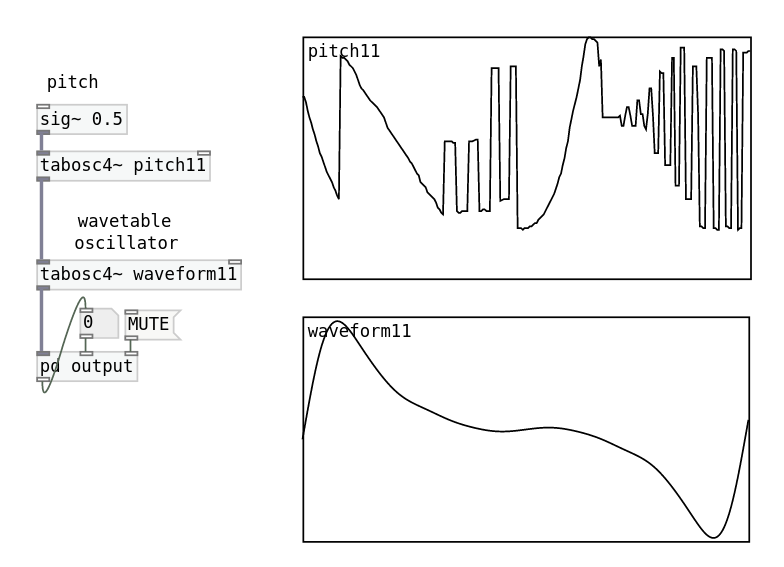
\includegraphics[width=1\textwidth]{./figuras/patch_puredata.png}
        \caption{Aspecto visual de un canvas de Pure Data}
      \end{subfigure}\hfill
    \source{Imagen del autor}
    \label{fig:patch_puredata}
\end{figure}



    
\section{El problema de componer con notas musicales}

Podemos incluir en nuestra lista sistemas de notación musical que se reducen a código, como Lilypond, la librería de Python Music21, ABC notation o el mismo formato MusicXML. Sin embargo, se ha podido comprobar desde un primer acercamiento a LLM como GPT-4, que aún no son capaces de generar un código mínimamente interesante artísticamente cuando hablamos de utilización de notas musicales, acordes, etc., a pesar de comprender perfectamente la sintaxis. La figura \ref{fig:melodia_bach} muestra una partitura generada por GPT-4, cuando se le pidió crear una melodía de 4 compases al estilo de Bach. Como se puede apreciar, la melodía es correcta desde el punto de vista de la sintaxis, pero no tiene ningún interés musical ni atisbo de aproximación estilística al la petición del usuario. Por tanto, se ha decidido excluir de esta investigación los lenguajes de notación musical.

\begin{figure}[h]
    \caption[Melodía de 4 compases generada por GPT-4, al estilo de Bach]{Melodía de 4 compases generada por GPT-4, al estilo de Bach. El LLM la entregó en formato Lilypond.}
    \centering
    \begin{subfigure}{.48\textwidth}
        \centering
        \begin{mdframed}
        \begin{verbatim}
\score {
    \new Staff {
        \key c \major
        \time 4/4
        \tempo 4 = 100
    
        % Compás 1
        c'4 d' e' g' |
    
        % Compás 2
        f' e' d' c' |
    
        % Compás 3
        e'4 f' g' a' |
    
        % Compás 4
        g' f' e' d' |
    }
    \layout { }
    \midi { }
    }
        \end{verbatim}
        \end{mdframed}
        \caption{Código Lilypond devuelto por GPT-4}
      \end{subfigure} \hfill

      \vspace{5mm} % Añade espacio vertical entre las filas

      \begin{subfigure}{.75\textwidth}
        \centering
        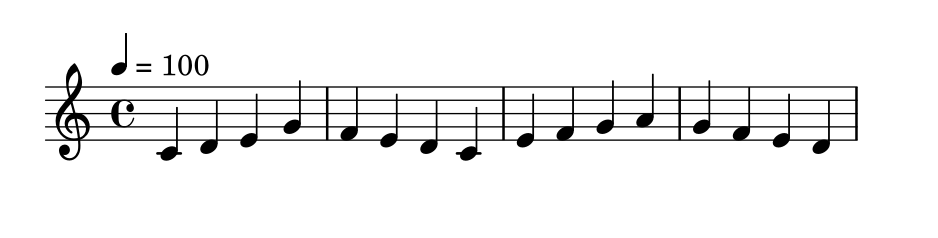
\includegraphics[width=1\textwidth]{./figuras/melodia_bach_estilo.png}
        \caption{Renderizado a notación musical por Lilypond}
      \end{subfigure}\hfill
    \source{Imagen del autor}
    \label{fig:melodia_bach}
\end{figure}

Este mismo problema lo encontramos en cualquier tipo de codificación que utilice notas musicales, como el formato MIDI.
Componer música con notas musicales, con las cotas de complejidad que ha alcanzado la música a lo largo del tiempo y de la geografía, no es una tarea trivial, y va mucho más allá del conocimiento básico de los simbolos utilizados en las diferentes notaciones. La música es un arte, y como tal, requiere de un conocimiento profundo de la teoría musical, de la armonía, del contrapunto, de la historia de la música, de la cultura musical, de la psicología de la percepción musical, etc. Es por ello que no podemos esperar que un LLM sea capaz de generar música con notas musicales de un modo interesante, al menos por el momento.

\section{Lenguajes orientados a la síntesis de sonido}

La música experimental, la música electrónica, la música electroacústica, la música concreta, la música generativa, etc., son géneros musicales que se han desarrollado en el siglo XX, y que han utilizado la tecnología como medio de expresión. En este contexto, han surgido numerosos lenguajes de programación orientados a la síntesis de sonido, que han permitido a los compositores de música electrónica y experimental crear sonidos y música de un modo más flexible y potente que con los sintetizadores analógicos \Citep{supperMusicaElectronicaMusica2012}. Estos lenguajes de programación han sido utilizados también en la creación de instalaciones sonoras, en la creación de interfaces de usuario o en la composición musical, y su desarrollo ha ido parejo con el de la tecnología digital. Una completa introducción al campo de la programación informática aplicada a la síntesis sonora es la de Curtis Roads (\citeyear{roadsComputerMusicTutorial1996}).

El lenguaje sonoro en torno a estos géneros musicales es mucho más flexible, por lo general, que el lenguaje de la música notada. Especialmente las músicas autodenominadas experimentales, que no tienen un lenguaje musical definido y que se caracterizan por la búsqueda de nuevos sonidos y nuevas formas de expresión, son idóneas para una experimentación con elementos no humanos, como los LLM. Esta interacción eventualmente puede traducirse en la exploración de nuevos timbres y texturas sonoras.

Dentro de los lenguajes de programación orientados a la síntesis de sonido, podemos distinguir entre los diseñados para ser codificados en interpretaciones en vivo, y los diseñados para ser codificados en archivos de audio, a una composición más estática. \textit{Csound} \citep{boulangerCsoundBookPerspectives2000} fue contruido para crear composiciones renderizadas en archivos de audio, si bien actualmente tiene características que le permiten ser ejecutado en tiempo real. \textit{SuperCollider} \citep{wilsonSuperColliderBook2011a} tiene características de ambos mundos, lo que lo hace óptimo tanto para la composición de obras sonoras como para la codificación en vivo, en lo que se denomina \textit{Live Coding}. Precisamente su ductilidad y potencia lo ha convertido en plataforma de audio sobre la que se han creado otros lenguajes orientados únicamente al tiempo real y \textit{Live Coding}, como \textit{FoxDot} (\citeyear{kirkbrideQirkyFoxDot2023}), \textit{Sonic Pi}, \textit{Overtone} (\citeyear{OvertoneCollaborativeProgrammable}) o \textit{Tidal Cycles} (\citeyear{LiveCodeTidal}). Actualmente proliferan lenguajes diseñados para esta interacción en tiempo real con el usuario. Además de los expuestos, podemos destacar \textit{ChucK} (\citeyear{teamChucKStronglyTimedMusic}) o \textit{Strudel} (\citeyear{StrudelREPL}), entre otros. Esto se debe, entre otros factores culturales, al aumento de la potencia de los ordenadores, que permite ejecutar en tiempo real programas de síntesis de sonido cada vez más complejos.

\section{Lenguajes seleccionados para esta investigación}

Hubiera sido de mucho interés incluir en esta investigación todos los lenguajes de programación musicales mencionados en este capítulo, y muchos más. Sin embargo, esto hubiera sido una tarea titánica, y hubiera requerido de mucho tiempo y recursos. Por ello, se ha decidido acotar la investigación a únicamente dos lenguajes de programación musicales, como punto de partida de ulteriores trabajos. En la elección se han tenido en cuenta una serie de criterios, que se exponen a continuación.


\subsection{Comunidad activa de usuarios y desarrolladores.} Se ha considerado importante que los lenguajes de programación musicales seleccionados tengan una comunidad activa de usuarios, que permita al investigador tener un soporte en caso de dudas o problemas. Esto es especialmente importante en el caso de los lenguajes de programación musicales, ya que no se trata de lenguajes de programación generalistas, sino de lenguajes de programación con un propósito específico, y por tanto, con una comunidad de usuarios más reducida que la de lenguajes de programación generalistas como Python o Java.

\subsection{Documentación extensa y accesible.} Una extensa y accesible documentación es crucial, no solo para que el investigador tenga una inmedita y fácil referencia de los elementos del lenguaje, de las librerías disponibles, de los ejemplos de código, etc., sino para que el LLM pueda tener acceso a esta documentación, y por tanto, pueda generar código de este lenguaje. Un momento crucial del entreamiento de los LLM es el preentrenamiento, en el que se les expone a todo tipo de texto, incluyendo código de programación. Cuanta más información de calidad exista en la red sobre un lenguaje de programación, incluyendo piezas musicales y tutoriales, más probable es que el LLM haya tenido acceso a ella, y por tanto, más probable es que sea capaz de generar código de este lenguaje.

\subsection{Capacidad de trabajo en tiempo real.} Es importante que los lenguajes de programación musicales seleccionados sean capaces de trabajar en tiempo real, ya que esto permitirá al investigador interactuar con el LLM en tiempo real, y por tanto, tener una experiencia más inmersiva y más rica. El uso de APIs permite una interacción continua y automatizada con los modelos de lenguaje. Como se ha señalado más arriba, prácticamente todos los lenguajes modernos tienen de uno u otro modo esta capacidad de ser ejecutados y codifiados en tiempo real, si bien algunos de ellos han sido creados con este objetivo en mente, como \textit{Sonic Pi} o \textit{Tidal Cycles}. El propio \textit{SuperCollider} posee la librería \textit{JITLib} (\textit{Just in Time Library}), que contiene toda la funcionalidad necesaria para la codificación en tiempo real.

Explicado de una forma rápida y sencilla, la codificación en tiempo real consiste en la ejecución de código de programación en tiempo real, en el momento de la interpretación. Esto permite al usuario interactuar con el código de un modo más inmediato, y por tanto, tener una experiencia más inmersiva. En el caso de los lenguajes de programación musicales, esto se suele conseguir creando bucles infinitos, que se ejecutan continuamente y pueden ser modificados en vivo (sustituidos) sin tener que reiniciar el programa, y permiten una intuitiva interacción con el usuario. La Figura \ref{fig:sonic_pi_loop} muestra un ejemplo de bucle infinito en \textit{Sonic Pi}. Este bucle es sustituido por otro nuevo en vivo cada vez que el usuario hace una modificación en él. No es difícil imaginar el papel que puede tener un modelo de inteligencia artificial en este proceso, generando código de programación sonora en tiempo real y permitiendo una interacción continua con el usuario, e incluso sin la intervención del usuario, como se verá más adelante.


\begin{figure}[h]
  \caption[Bucle infinito en \textit{Sonic Pi}]{Bucle infinito en \textit{Sonic Pi}. En este código se ejecutan cuatro notas, una por segundo en un bucle infinito. El usuario puede modificar las notas, y el cambio se ejecuta en el siguiente ciclo del bucle.}
  \centering
  \begin{subfigure}{.5\textwidth}
  \begin{mdframed}
  \begin{verbatim}
  live_loop :melody do
    play :E4
    sleep 1
    play :G4
    sleep 1
    play :B4
    sleep 1
    play :C5
    sleep 1
  end
  \end{verbatim}
  \end{mdframed}
  \end{subfigure}
  \source{Elaboración del autor en \textit{Sonic Pi}}.
  \label{fig:sonic_pi_loop}
\end{figure}

\subsection{Fácil gestión de errores.} En el proceso de depuración de un código, incluido el de una pieza musical, es eminentemente iterativo. Se prueba el código, se detectan errores, se corrigen, se vuelve a probar, etc. Es importante que el lenguaje de programación musical permita una depuración rápida y eficiente, para que el investigador pueda centrarse en la creación musical, y no en la depuración del código. Esto es especialmente importante en el caso de los LLM, ya que estos no son capaces de detectar errores en el código, y por tanto, el investigador debe ser capaz de detectarlos y corregirlos de un modo rápido y eficiente.

Esta característica está muy unida a la anterior, ya que un buen lenguaje con capacidades de tiempo real ha de ser inmune a los errores. Si en una iteración el usuario comete un error, el programa no debe detenerse, sino que debe continuar ejecutándose, y el usuario debe ser capaz de corregir el error y continuar con la iteración. Los LLM, al igual que los músicos humanos, cometen errores, y en las interpretaciones en vivo estos errores deben ser ignorados en muchas ocasiones en pro de la fluidez de la sesión. En el caso de una composición renderizada en un archivo de audio, los errores deben ser corregidos antes de la renderización, y el proceso de depuración es más lento y minucioso. En este caso no es crítico que el lenguaje de programación sea inmune a los errores. Al contrario, es importante que devuelva mensajes de error claros y precisos, para que el investigador pueda corregirlos de un modo rápido y eficiente. 

\textit{SuperCollider} es un ejemplo que une ambos mundos. Cuando se usa la librería \textit{JITLib}, el código se ejecuta en tiempo real, y el usuario puede concentrarse en la creación musical, y no tanto en la depuración del código. Si lo que se desea es crear una composición separada del momento interpretativo, su consola de errores es muy precisa y permite una depuración rápida y eficiente.

\textit{Tidal Cycles}, que está enfocado principalmente a la codificación en tiempo real (o \textit{Live Coding}), permite una ejecución sonora continua por defecto, abstraido completamente de los errores. El artista ha de estar atento a la consola para detectar los errores, pero será muy raro que el software termine su ejecución por un error. Esta es una característica muy interesante para la interacción con LLM, asegurando que no existirán interrupciones indeseadas ante código erróneo o respuestas inesperadas del modelo.

\subsection{Independencia del IDE}
Esta característica es importante si se quiere utilizar un LLM por medio de la API. Si un lenguaje tiene un apropia interfaz gráfica o IDE (\textit{Integrated Development Environment}), no hay un modo sencillo de ejecutar dicho código por medio de scripts creados ad hoc con Python u otros lenguajes de programación. Una investigación profunda en la interacción entre LLM y usuario humano requiere de un control total sobre el código que se le pasa al LLM, así como la posibilidad de automatizar la ejecución del código y convertirlo en sonido a través de scripts o software creado ad hoc. Por ello, se ha considerado importante que los lenguajes de programación musicales seleccionados no tengan un IDE propio, o que este IDE no sea imprescindible para la ejecución del código. Un ejemplo de utilización de IDE propio es \textit{Sonic Pi}, que no permite por defecto la ejecución de código por medio de scripts externos. \textit{SuperCollider}, aunque tiene un IDE propio, su intérprete de comandos, \textit{sclang}, puede ser ejecutado por medio de scripts externos, y por tanto, es independiente de IDE. Esta característica de independencia del IDE utilizado es heredado por lenguajes que usan \textit{SuperCollider} como motor de sonido, como \textit{FoxDot} o \textit{Tidal Cycles}.

\subsection{Lenguajes dominados por el investigador.} 
Quizás sea este el más arbitrario de todos los criterios, pero un desnivel de conocimiento entre lenguajes podría sesgar los resultados de la investigación. En este caso, el investigador tiene amplia experiencia con \textit{SuperCollider}\footnote{Véase el trabajo previo del propio autor \citep{guerraparraMesjetiuTFM_Arte_Sonoro_MEMORIA2020}.}, \textit{Csound}, \textit{Tidal Cycles} y \textit{Sonic Pi}.
Es importante que el investigador domine los lenguajes de programación musicales seleccionados, para poder centrarse en la creación musical, y no tanto en la depuración del código. Esto es especialmente importante en el caso de los LLM, ya que estos no son capaces de detectar errores en el código, y por tanto, el investigador debe ser capaz de detectarlos y corregirlos de un modo rápido y eficiente.

\subsection{\textit{SuperCollider} y \textit{Tidal Cycles}}
Se ha decidido utilizar \textit{SuperCollider} y \textit{Tidal Cycles} como lenguajes de programación musicales para esta investigación. Ambos lenguajes cumplen sobradamente con los criterios expuestos. Se trata de lenguajes muy potentes y flexibles, suficientemente conocidos por el investigador y con una comunidad activa de usuarios y desarrolladores. Ambos soportan un trabajo fluido en tiempo real, aunque enfocaremos la creación de código para piezas musicales en \textit{SuperCollider} principalmente, y el trabajo que implique codificación en tiempo real, en \textit{Tidal Cycles}. Ambos lenguajes son independientes del IDE, y por tanto, pueden ser ejecutados por medio de scripts externos por medio de scripts en Python. Véase la Tabla \ref{tab:lenguajes_comparativa} para una comparativa de los lenguajes de programación musicales en función de los criterios expuestos. Dicha tabla no es exhaustiva. Una lista más completa de lenguajes de programación musicales puede encontrarse en \cite{ListAudioProgramming2023}

\begin{table}[h] % t de top
  \begin{center}
  \caption[Lenguajes de programación musicales más relevantes]{Lenguajes de programación musicales más relevantes. El número de desarrolladores se ha obtenido de la página de GitHub de cada lenguaje. La documentación y el nivel de \textit{Live} se han valorado de 1 a 3 asteriscos, siendo 3 asteriscos la máxima puntuación.}
  \begin{tabular}{| c | c | c | c | c | c | c |}
  \hline
  Lenguaje & Lanzamiento & Actualización & Desarrolladores & Documentación & \textit{Live} & Independiente de IDE\\
  \hline
  \textit{Csound} & 1985 & 2022 & 56 & *** & * & Sí\\
  \textit{SuperCollider} & 1996 & 2023 & 212 & *** & ** & Sí\\
  \textit{ChucK} & 2003 & 2023 & 44 & *** & ** & Sí\\
  \textit{Tidal Cycles} & 2009 & 2023 & 76 & *** & *** & Sí\\
  \textit{Overtone} & 2010 & 2023 & 68 & ** & ** & Sí\\
  \textit{Sonic Pi} & 2012 & 2023 & 532 & *** & *** & No\\
  \textit{FoxDot} & 2019 & 2021 & 35 & * & *** & Sí\\
  \textit{Strudel} & 2022 & 2023 & 29 & *** & *** & No\\

  \textit{GLICOL} & 2022 & 2023 & 29 & *** & *** & No\\ % poner datos reales y comentar
  \textit{FAUST} & 2022 & 2023 & 29 & *** & *** & No\\ % poner datos reales y comentar
  \hline
  \end{tabular}
  \source{Elaboración del autor en \textit{Sonic Pi}}.
  \label{tab:lenguajes_comparativa}
  \end{center}
\end{table} 